\section{RethinkDB}

This chapter briefly introduces the major topics around RethinkDB, a real time open source shema-less document-based database. It is widely used by startups and Fortune 500 firms such as NASA, GM and Distractify. Founded in 2009 RethinkDB saw major funding by Y Combinator, had their first release 2012 and went to version 2.0 in 2015. October 2016 the company behind RethinkDB closed down due to the lack of business success but the software got then purchased in February 2017 by a Linux Foundation daughter: The Cloud Native Computing Foundation. It has then been re-licenced under Apache Licence 2.0, going away from their initial copyleft-like licence \cite{RethinkCNCF,techcrunchredb}.   

\section{How RethinkDB works}

\subsection{Data storage in Rethinkdb}

\subsubsection{The data structure}

RethinkDB stores data as a B-tree-structure. A B-tree is a data structure which is balancing itself and allows filtering and sorting within logarithmic time. This B-tree is saved on a file system instead of the RAM in large structures \cite{BTreeTechTarget}. This file system is called BTRFS (B-Tree File System),  This enables the copy-on-write scheme provided by BTRFS thus making it possible to repair saved data from the copied clone. Other benefits to this filesystem are a garbage compactor to reduce older copies, low cpu-overhead, optimization for solid-state drives, data consistency (more detail about consistency in the ACID and CAP chapter \ref{acidcap} , b-tree aware caching and multi version control\ref{mvcc}. B-Tree aware caching is a way to give RethinkDB the capability of using far more data than available RAM.\\
RethinkDB does not include a hardware data consistency, this has to be maintained by the used file system itself, which RethinkDB supports the most commonly available \cite{RethinkDataStorage}


\subsubsection{partioning and multi-datacenter support}

Data in RethinkDB can be saved on multiple servers. This is done by replicating databases and providing each of them with a specific tag such as 'de\_east' or 'westeros'. A table can have an non-specific amount of replicas on each server. 
On servers data can be partitioned into shards and furthermore tagged like replicas.  The partition is done by a range of specific sharding algorithms and uses the primary key of each table. This means, that a shard key and a primary key is identical. For example if a data set has a primary key containing only letters and is ordered alphabetical, the sharding algorithm will likely split the data around the key 'm'. Thus the new two partitions containing every data with a key from 'a' to 'm' and from 'n' to 'z'. Evidently this algorithm always tries to part at the best pivot to have new partitions in equal size.\cite["How does multidata-center support work"]{RethinkSharding}

\subsection{The atomicity model}
\label{atomicity}
Atomicity means, that either the complete stack of operations will be executed or non at all, there is no middle ground \cite{TechTargetAcid}.
Operations within single json documents are guaranteed to be atomic, queries accessing different keys are not as they may be inconsistent in read and write operations \cite{jepsen2016}.
The atomicity differs itself from other NoSQL databases by the way, that every set of operations, every chained query is atomic by the restriction named above. Plus, another limit is, that upon executing a non deterministic operation RethinkDB will nolonger be able to ensure their atomicity. In this case, RethinkDB will automatically throw an error by default. This behaviour may be shut by setting the according flag \cite["How does atomicity work"]{RethinkQE}.  

\subsection{ACID and CAP theorems in RethinkDB}
\label{acidcap}
RethinkDB’s architecture is based, as mentioned in the section above \ref{atomicity}, on the atomicity model. This model is part of the ACID paradigm for databases. ACID is a acronym for atomicity, consistency, isolation, and durability and describes the key desired parameters during a transaction to and off of a Database. ACID is norminized under ISO/IEC 10026-1:1992 Section 4 \cite{TechTargetAcid}. 
RethinkDB has also support for every other ACID paradigm except full isolation and absolute data consistency and therefore might not the best choice if full ACID-Support is needed. But RethinkDB provides a basic consistency as specified within the CAP-theorem. What this theorem is, has been elaborated within the Architectural Basics of Cassandra \ref{captheroem}. The basic consistency within RethinkDB has been ensured by the fact, that every shard has a single replication and read and write actions are performed on this replication but not on the shard itself. Data remains immediately consistent and conflict-free. 
The Database also provides availability needed by the CAP-theorem as data is also accessible both up-to-date and out-of-date. Out-of-date queries are executed on a snapshot and without trying to get the most current data set. This means, that these queries are faster and guarantee availability but may not return nor access the most current data. The up-to-date queries are assuring that they return the latest data consistent and artifact-free. As before mentioned data is not absolutely consistent. This tradeoff roots within the partitioning. RethinkDB assures data to be consistent on the same network but cannot do the same for network partitions if data has to be up-to-date.\cite{RethinkCAP}. 

\begin{figure}[H]
	\begin{center}
		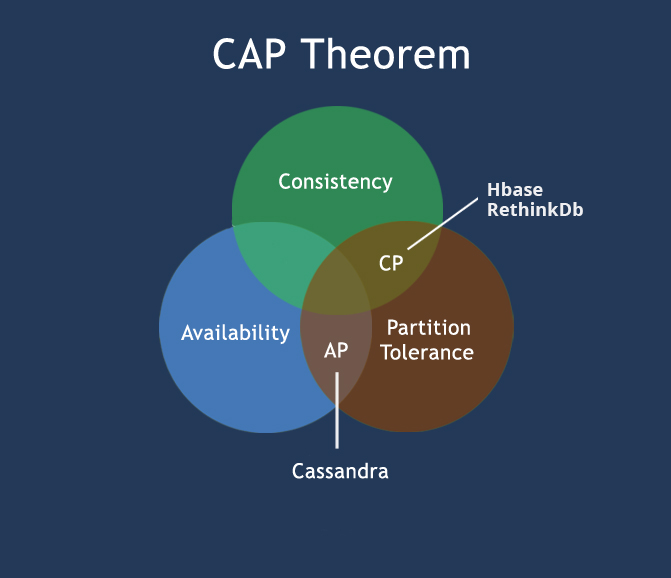
\includegraphics[scale=0.6,keepaspectratio]{images/captheoremnosql.jpg}
		\caption{Position of RethinkDB in the CAP-Theorem \protect\cite{rdbcaptheorem}}
	\end{center}
\end{figure}

\subsection{multiversion concurrency control}
\label{mvcc}

RethinkDB has built-in support for multi version concurrency control. This means, that every writing operation is by default only made after a snapshot, simply a read operation, has been taken off of that tree. This has following benefits:
\begin{itemize}
	\item Easy roll backing to previous data
	\item Lock-Free read and write operations
	\item Enables non-blocking queries making real-time hour long possible
\end{itemize}
\cite["How are concurrent queries handled?
"]{RethinkQE}

\section{The query language ReQL}

RethinkDB has its own query language called ReQL. A query contains the table, an action and the order to run on a specific database connection. For Example the query to get an id (1) from a table (test) looks like this:

\begin{lstlisting}[frame=single, caption=get document from Database  (javascript driver), label=rget]
r.table("test").get(1).run(connection)
\end{lstlisting}

One idiomatic aspect of ReQL is already evident in this example. ReQL is a chain of commands. Multiple queries can be written as a one-liner and are thus executed as one without disturbance. If there are dependencies on another query one should use this chain-technique to make sure it is executed in the right order. This works due to the fact, that the query is only parsed and executed on the server while being build on the client. On top of that, RethinkDB is lazy executing the queries.  It immediately stops upon satisfaction. 
Furthermore are those queries functional and allows adding lambda functions as parameter. RethinkDB has build-in support for example for javascript code through the V8-Engine, map-reduce, table-joins and math \cite{reql}.

\begin{lstlisting}[frame=single, caption=create the table 'test', label=createTable]
r.db("test").tableCreate("test", options).run(connection)
\end{lstlisting}

Every table created gets a primary key for indexing. By default it is id but this can be changed by providing an option:
\begin{lstlisting}[frame=single, caption=options for create table, label=cTableOptions]
{primaryKey: 'name'}
\end{lstlisting}

By setting this option as in the example, the table now is indexing every row under „name“.
TableCreate has, as most of the  many different options available, accessible in their documentation \cite{tableCreate}. 

\subsection{query executing}

RethinkDB has a special way of executing a query. One key point is, that the query is not executed on a client but on the server itself. By receiving the query, the server creates a list of instructions consisting of internal logical operations. RethinkDB now tries to make this list as efficient as possible by executing most basic operations first and more time consuming, such as manipulating data last. Each operation set is called Node and their complexity ranges from single document queries to deep complex subquery commands. After executing, the server returns his result as a datastream not only to the client itself but also to every other relevant server. This has the benefit, that RethinkDB does not really care on which server the query is executed and therefor can parallize this process.
\cite["How does RethinkDB execute queries?"]{RethinkQE}

\section{RethinkDB perfomance analysis}

RethinkDB had has a major performance issue since its start but kept on improving on this aspect over the years. For example in a comparison in 2014, MongoDB has been 3 times faster than RethinkDB at executing queries over a large patent data set\cite{rvsm2014}.
A newer comparison of 2015 turns this around but only for writing data to the database. Reading, RethinkDB has still been half as fast as MongoDB has been in that benchmark\cite{rvsm2016}.
Within an official benchmark test, the RethinkDB Team got this result:

\begin{figure}[H]
	\begin{center}
		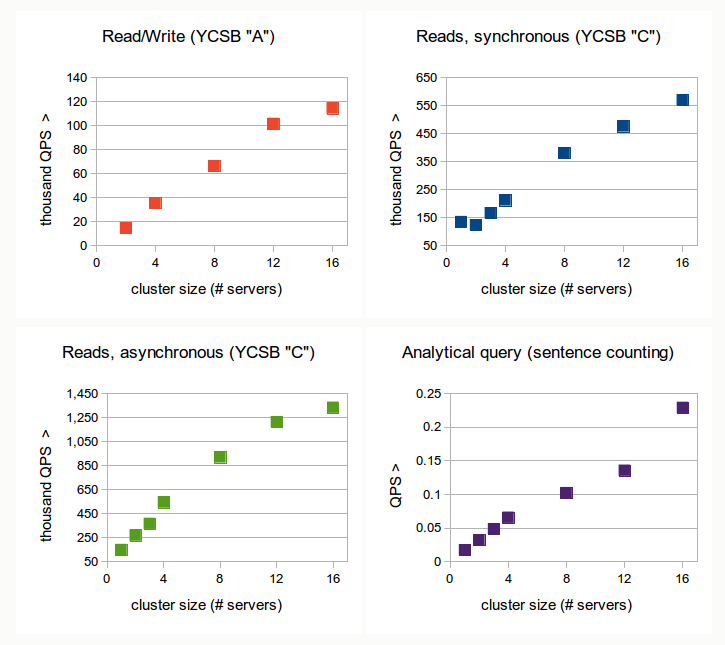
\includegraphics[scale=0.6,keepaspectratio]{images/performanceReport.png}
		\caption{Performance Report of RethinkDB \protect\cite{performanceReport}}
	\end{center}
\end{figure}

They states, that in their working environment they were able to perform around 16 000 queries in a second (QPS). For this benchmark, RethinkDB used "analytic workloads in a simplistic but very common fashion" \cite{performanceReport}.